\documentclass[11pt,a4paper]{article}
\usepackage{fontspec}
\usepackage{xeCJK}
\setmainfont[Path=/mnt/c/Windows/Fonts/,BoldFont=timesbd.ttf,ItalicFont=timesi.ttf,BoldItalicFont=timesbi.ttf]{times.ttf}
\setmonofont[Path=/mnt/c/Windows/Fonts/,BoldFont=consolab.ttf,Scale=0.88]{consola.ttf}
\setCJKmainfont[AutoFakeBold=2]{WenQuanYi Zen Hei}
\setCJKsansfont[AutoFakeBold=2]{WenQuanYi Zen Hei}
\setCJKmonofont[Scale=0.88]{WenQuanYi Zen Hei Mono}
\usepackage[margin=2.2cm]{geometry}
\usepackage{graphicx,float,booktabs,tabularx,array,enumitem,fancyvrb,url,caption}
\usepackage{xcolor}
\usepackage{tikz}
\usetikzlibrary{arrows.meta,positioning,fit}
\usepackage[colorlinks=true,linkcolor=blue!50!black,urlcolor=blue!50!black]{hyperref}
\linespread{1.25}
\setlength{\parindent}{2em}
\setlength{\parskip}{3pt}
\setlist{itemsep=2pt,topsep=3pt}
\captionsetup{font=small}
\renewcommand{\figurename}{图}
\renewcommand{\tablename}{表}
\renewcommand{\contentsname}{目录}
\renewcommand{\abstractname}{摘要}
\setcounter{tocdepth}{1}
\newcommand{\code}[1]{\texttt{\detokenize{#1}}}
\fvset{fontsize=\small,frame=single,framesep=6pt,rulecolor=\color{black!30}}
\newcolumntype{Y}{>{\raggedright\arraybackslash}X}

\title{\textbf{摄像头人体动作模仿：Robotis MINI 仿真与真机}\\[4pt]\large Final Project 中期 Report}
\author{Xiang Li}
\date{2026 年 10 月 31 日}

\begin{document}
\maketitle
\thispagestyle{empty}

\begin{abstract}
\noindent
本项目用一个普通摄像头识别人体姿态（MediaPipe），把人的手臂和腿的动作实时映射到 Robotis MINI 人形机器人的 16 个关节上，先在 MuJoCo 仿真中完成，再迁移到装有 KIMLAB 升级套件的真机上。系统包括：WSL2 下的摄像头接入与 Windows 推流、基于肢体方向的关节重定向、启动保护与平滑、静态重心安全过滤，以及通过 U2D2 驱动 XL-320 舵机的真机桥接节点。仿真中，端到端延迟从“越积越多、数秒以上”降到约 0.25 秒；加入重心安全过滤后，抬膝、迈步、下蹲等 6 种测试动作在物理仿真中全部站稳，而不加过滤时其中 5 种会摔倒。真机已完成通信、关节方向与零点校准，并完成一次 77 秒的全身实时模仿运行；电池电压是目前真机长时间运行的主要限制。
\end{abstract}

\tableofcontents
\newpage

%=====================================================================
\section{项目概述}

\subsection{目标}
让机器人实时模仿摄像头前人的动作：人抬手，机器人抬手；人抬膝，机器人在不摔倒的前提下抬膝。左右按“左对左”对应：人的左臂驱动机器人的左臂。

\subsection{整体结构}
整个系统是一条从摄像头到关节的流水线（图~\ref{fig:pipeline}）。仿真和真机共用前面所有环节，只有最后一步不同：仿真时命令发给 MuJoCo 仿真器，真机时发给桥接节点，再由 U2D2 转发给舵机。两者订阅的是同一个 ROS 话题，所以模仿节点本身不用做任何修改。

\begin{figure}[H]
\centering
\begin{tikzpicture}[
  node distance=5mm and 6mm,
  box/.style={draw, rounded corners=2pt, align=center, font=\small, minimum height=10mm, inner sep=4pt, fill=blue!4},
  outbox/.style={box, fill=orange!8},
  arr/.style={-{Stealth[length=2.2mm]}, thick}]
\node[box] (cam) {摄像头\\\scriptsize 笔记本 / Windows 推流};
\node[box, right=of cam] (mp) {MediaPipe\\\scriptsize 33 个关键点};
\node[box, right=of mp] (rt) {重定向\\\scriptsize 启动保护 + 平滑};
\node[box, right=of rt] (bf) {重心安全过滤\\\scriptsize 腿部命令};
\node[font=\scriptsize, align=center, below=11mm of bf] (topic) {\code{/robotis_mini/whole_body_controller/command}};
\node[outbox, below left=10mm and -8mm of topic] (sim) {MuJoCo 仿真\\\scriptsize \code{mujoco_ros_interface}};
\node[outbox, below right=10mm and -8mm of topic] (real) {真机桥接节点\\\scriptsize U2D2 $\rightarrow$ 16 个 XL-320};
\draw[arr] (cam) -- (mp); \draw[arr] (mp) -- (rt); \draw[arr] (rt) -- (bf);
\draw[arr] (bf) -- (topic);
\draw[arr] (topic) -- (sim); \draw[arr] (topic) -- (real);
\node[draw=black!40, dashed, rounded corners, fit=(cam)(mp)(rt)(bf), inner sep=5pt, label={[font=\scriptsize]above:\code{pose_imitation.py}（仿真与真机共用）}] {};
\end{tikzpicture}
\caption{系统流水线。虚线框内是模仿节点，仿真和真机完全相同。}
\label{fig:pipeline}
\end{figure}

\subsection{运行环境}
\begin{itemize}
  \item Windows 笔记本 + WSL2（Ubuntu 20.04），ROS Noetic，Python 3.8。
  \item MediaPipe 0.10.11（Python 3.8 能用的最后一个版本；它依赖的 jaxlib 在 PyPI 上已没有 3.8 的版本，所以用 \code{--no-deps} 安装再手动补齐依赖），OpenCV（opencv-contrib-python 4.10）。
  \item MuJoCo 3.1.4 装在仿真包自带的虚拟环境（\path{robotis_mini_mujoco/.venv}）里，由仿真器使用。
  \item USB 设备（摄像头、U2D2）通过 Windows 上的 usbipd-win 挂进 WSL。
\end{itemize}

%=====================================================================
\section{代码结构}
所有 final project 的代码都在独立的 ROS 包 \path{~/ws_mini/src/final_project} 中，没有修改 assignment2 的任何文件；仿真器和机器人模型直接复用 assignment2 仓库里的包（只读）。

\begin{table}[H]
\centering\small
\begin{tabularx}{\textwidth}{>{\ttfamily}p{6.1cm}Y}
\toprule
\normalfont 文件 & 作用 \\
\midrule
src/pose\_imitation.py & 模仿节点：读摄像头、MediaPipe 识别、重定向、重心过滤、发布关节命令；可选记录每帧数据 \\
src/pose\_retarget.py & 重定向（纯 numpy，可离线测试）：关键点 $\rightarrow$ 16 个关节角，含启动保护和平滑 \\
src/balance\_filter.py & 静态重心安全过滤：移重心、抬腿保护、限制下蹲深度 \\
src/windows\_stream.py & 接收 Windows 推流的 JPEG 帧，只取最新一帧 \\
src/real\_robot\_bridge.py & 真机桥接：关节命令 $\rightarrow$ XL-320 舵机，读回关节角，电压/温度保护 \\
config/mujoco\_sim.yaml & 仿真器配置副本（只关闭了没用到的机器人头部摄像头渲染） \\
config/mini\_mass\_model.json & 机器人各部件质量、质心、脚底轮廓（从 MuJoCo 模型导出） \\
config/real\_robot\_calibration.yaml & 真机关节对照：舵机 ID、方向、零点 \\
launch/mujoco\_imitation.launch & 仿真 + 模仿 \\
launch/real\_imitation.launch & 真机桥接 + 模仿 \\
tools/ & 录屏、数据提取与分析、仿真回归测试、舵机扫描与校准等工具（见第~\ref{sec:tools}~节） \\
\bottomrule
\end{tabularx}
\caption{\code{final_project} 包的主要文件}
\end{table}

\noindent 另外，\path{~/ws_mini/vision/} 中的 \code{human_pose.py} 是最初的独立骨骼识别脚本，\code{win_camera_sender.py} 是 Windows 端的摄像头推流程序。

%=====================================================================
\section{摄像头接入}

\subsection{笔记本自带摄像头}
WSL2 默认看不到 USB 摄像头。做法是在 Windows 上用 usbipd 把摄像头挂进 WSL：
\begin{Verbatim}
usbipd bind --busid 1-3 --force     # 管理员 PowerShell，只需做一次
usbipd attach --wsl --busid 1-3     # 每次重启电脑 / WSL 后做一次
\end{Verbatim}
挂载后 WSL 里出现 \code{/dev/video0}。通过 usbip 传输时带宽有限，未压缩的 YUYV 格式会读帧超时，所以程序里把格式设为 MJPG、640$\times$480。用户还需要加入 \code{video} 组才有权限读摄像头。

\subsection{外接 USB 摄像头（Windows 推流）}
外接的 USB 2.0 PC Cam 只支持未压缩的 YUYV 格式，经 usbip 传输时大量丢包（内核日志中有大量 \code{urb->status -104}），画面只有顶部十几行，其余全是绿色。降低分辨率、单独挂载、调整 uvcvideo 参数都没有用。最终方案是不经过 usbip：在 Windows 上用 OpenCV 采集画面，压缩成 JPEG，通过 TCP（端口 5600）推给 WSL。
\begin{Verbatim}
python.exe "$(wslpath -w ~/ws_mini/vision/win_camera_sender.py)" \
    0 $(hostname -I | cut -d' ' -f1)
\end{Verbatim}
有两点需要注意：
\begin{itemize}
  \item \textbf{连 WSL 的 IP，不要连 127.0.0.1。} 127.0.0.1 依赖 Windows 的 wslrelay 转发，测试中它出现过“接受连接却不转发”的情况：推流端显示已连接，WSL 端却一直收不到画面。
  \item \textbf{接收端只处理最新一帧。} 摄像头每秒送来的帧比识别能处理的多时，按顺序处理会让旧帧在网络缓冲区里越积越多。改为每次读取时清空缓冲区、只取最后一帧之后，画面“年龄”稳定在 0.01–0.04 秒（第~\ref{sec:latency}~节）。
\end{itemize}

%=====================================================================
\section{姿态识别与重定向}

\subsection{识别}
MediaPipe Pose Landmarker（\code{pose_landmarker_full.task}，VIDEO 模式，单人）每帧输出 33 个关键点的图像坐标、三维世界坐标和可见度。重定向只用 12 个身体关节点（肩、肘、腕、髋、膝、踝），手指、脚趾和脸部的点不用。

\subsection{重定向方法}
\begin{enumerate}
  \item \textbf{人的躯干坐标系}：用左右肩和左右髋算出人的躯干朝向（前、左、上），把每段肢体（上臂、前臂、大腿、小腿）的方向换算到躯干坐标系里。这样人整体转身或前倾时，手臂相对身体的动作不受影响。
  \item \textbf{逐肢体求关节角}：机器人坐标系是 x 向前、y 向左、z 向上。每条手臂 3 个关节（肩、上臂、肘），每条腿取前 3 个关节（髋侧摆、大腿、膝），用最小二乘（带关节限位）求出让机器人肢体方向最接近人的关节角。上一帧的结果作为初值，拟合不好时再换其他初值，避免卡在错误的解上。每帧计算约 7.5 ms。
  \item \textbf{脚底保持水平}：踝关节 = 大腿 + 膝，脚侧摆 = 髋侧摆，使脚底始终平行于躯干，有利于站稳。
  \item \textbf{验证}：自己写的运动学与 MuJoCo 模型在随机 200 组关节角下的肢体方向误差为 $10^{-15}$ 量级；10 种标准姿势的重定向误差除一种外均为 0°。
\end{enumerate}

\paragraph{机器人结构限制} MINI 的手臂在肩关节转动之后，上臂和前臂只能在同一个平面内运动，而这个平面总是包含机器人的左右方向。因此“上臂下垂、前臂向前伸”这类动作做不出来，求解器只能给出最接近的姿势（测试中误差约 26°/64°）。

\subsection{启动保护与平滑}
\begin{itemize}
  \item \textbf{启动保护}：启动后先保持默认站姿，等到全身（肩、髋、膝、踝）都在画面内、且人是站着的（大腿接近竖直），连续约 1 秒后，再用约 1 秒从站姿过渡到人的姿势。腿部关键点除了可见度要够，还必须在画面范围内，因为 MediaPipe 会对画面外的腿给出看起来可信的猜测。
  \item \textbf{平滑}：对关节命令做指数平滑（权重 0.3），并限制每帧最大变化 0.4 rad。看不清的肢体保持上一次的姿势。
\end{itemize}

%=====================================================================
\section{重心安全过滤}
\label{sec:balance}

\subsection{为什么需要}
早期测试中，所有离地的腿部动作都会让机器人摔倒，原因有两类：
\begin{itemize}
  \item \textbf{重心没有移到支撑脚上方}：人抬腿前会先把重心移到另一只脚，机器人只照抄腿的角度，脚一离地就倒。
  \item \textbf{膝关节力矩不够}：机器人上身保持直立，深蹲时膝盖远在髋关节前方，起身需要的膝关节力矩超过 XL-320 的 0.39 Nm 上限，膝盖伸不直，机器人向后倒。
\end{itemize}

\subsection{方法}
过滤器位于重定向之后、发布命令之前，每帧只修改腿部关节：
\begin{enumerate}
  \item \textbf{计算重心}：用从 MuJoCo 模型导出的质量参数（\code{mini_mass_model.json}），在“躯干直立、脚底水平”的假设下算出整机重心和两只脚的脚底轮廓（每只脚 84~mm $\times$ 48~mm）。与 MuJoCo 对比误差为 0，一次计算约 0.2 ms。
  \item \textbf{判断支撑脚}：两脚高度差小于 10~mm 时视为识别抖动，把较高的那只脚压回地面，保持双脚支撑；超过 10~mm 进入单脚支撑，回到 5~mm 以下才恢复双脚（滞回，防止来回切换）。
  \item \textbf{先移重心再抬腿}：单脚支撑时，两条腿一起侧摆、一起前后倾（脚底保持水平），把重心移到支撑脚脚底边缘内侧（留 8~mm 余量）。只移到边缘内侧而不是正中间，侧摆角度从约 26° 降到约 15°，髋关节舵机才扛得住。重心移到位之前，抬起的那条腿保持在地面上。
  \item \textbf{限制下蹲深度}：着地的腿大腿前倾最多 30°（超过时髋和膝按同一比例缩小）。仿真测试表明 30° 以内可以正常站起，40° 就会因膝关节力矩不够而倒下。
  \item \textbf{兜底}：上述步骤后仍不安全时，把腿往默认站姿收，直到安全为止。
\end{enumerate}
这是静态检查，前提是动作比较慢；快速抬腿、踢腿仍可能摔倒。

\subsection{仿真测试结果}
测试方法：用合成的人体关键点生成慢速动作（2 秒到位、保持 3 秒、2 秒复原），经过重定向（和过滤）后，在 MuJoCo 物理仿真中按 20 Hz 执行，统计躯干最大倾斜，超过 45° 视为摔倒。

\begin{table}[H]
\centering\small
\begin{tabular}{lcc}
\toprule
测试动作 & 不加过滤 & 加过滤 \\
\midrule
抬左膝 70° & 2.0 s 摔倒 & 站稳（6°） \\
抬右膝 70° & 2.0 s 摔倒 & 站稳（5°） \\
左腿前迈 30° & 3.0 s 摔倒 & 站稳（7°） \\
右腿侧抬 40° & 站稳（7°） & 站稳（12°） \\
深蹲（大腿 80°） & 6.5 s 摔倒 & 站稳（4°，下蹲压缩到 47\%） \\
中蹲（大腿 40°） & 6.3 s 摔倒 & 站稳（4°） \\
\midrule
重放实际录制的动作（75 s） & 56.7 s 摔倒（弯腰） & 全程站稳（最大 6°） \\
\bottomrule
\end{tabular}
\caption{重心安全过滤的仿真测试（括号内为躯干最大倾斜）}
\end{table}
\noindent 在重放实际录制数据时，站着不动的识别抖动会让两脚目标高度相差最多约 5~mm。加入“10~mm 以内视为抖动、把较高的脚压回地面”的处理后，被误判为单脚支撑的帧从 39\% 降到 0。

%=====================================================================
\section{仿真运行}

\subsection{启动方法}
\begin{Verbatim}
# 终端 1：仿真 + 模仿（外接摄像头经 Windows 推流）
cd ~/ws_mini && source devel/setup.bash
roslaunch final_project mujoco_imitation.launch camera_source:=win
# 终端 2：Windows 端推流
cd ~/ws_mini/vision
python.exe "$(wslpath -w win_camera_sender.py)" \
    0 $(hostname -I | cut -d' ' -f1)
\end{Verbatim}
常用参数：\code{camera_source:=0} 使用笔记本自带摄像头（不需要终端 2）；\code{imitate_legs:=false} 只模仿手臂；\code{balance_filter:=false} 关闭重心过滤；\code{log_file:=<路径>.npz} 记录每帧数据。摄像头窗口左上角显示状态：\code{no person}、等待全身入镜、\code{starting}（过渡中）、\code{tracking}，以及支撑状态 \code{[support: double/l/r]}。在 MuJoCo 窗口按 Backspace 可以复位机器人。

\subsection{延迟分析}
\label{sec:latency}
用仿真运行 \code{20261031_170832} 的数据，把各环节的延迟分开测量。“改前”用同一份数据推算（按顺序处理的推算假设队列可以无限变长，实际会被网络缓冲区上限卡住，但同样越积越多）。

\begin{table}[H]
\centering\small
\begin{tabular}{lcc}
\toprule
环节 & 改前 & 改后 \\
\midrule
网络传输（画面“年龄”） & 越积越大，60–80 s 时约 22 s & 0.02 s \\
平滑 & 60 ms & 20 ms \\
图像识别（MediaPipe 等） & 52 ms & 52 ms \\
机器人关节跟上命令（仿真内部） & 155 ms & 155 ms \\
\midrule
合计 & 数秒且不断增大 & 约 0.25 s \\
\bottomrule
\end{tabular}
\caption{端到端延迟（Windows 端采集、压缩和传输未计入）}
\end{table}
\noindent 剩下最大的一项是关节跟随（约 100 ms 来自每条命令 0.1 s 的过渡时间，其余是仿真关节本身的响应速度）。

\subsection{运行效果}
图~\ref{fig:sim} 是仿真运行 \code{20261031_174418}（带重心过滤）的录屏截图，左边是 MuJoCo，右边是摄像头画面。这次运行中有 3 次单脚支撑（左脚 28.1–32.1 s，右脚 36.4–40.2 s，左脚 63.4–65.1 s），机器人都先移了重心再抬腿，没有摔倒；同样的动作不加过滤时，离线重放在第一次抬膝（29.9 s）就会摔倒。第 73.4 s 从深蹲快速起身（不到 1 秒）时摔倒了一次，这是目前还没有处理的情况（第~\ref{sec:limits}~节）。

\begin{figure}[H]
\centering
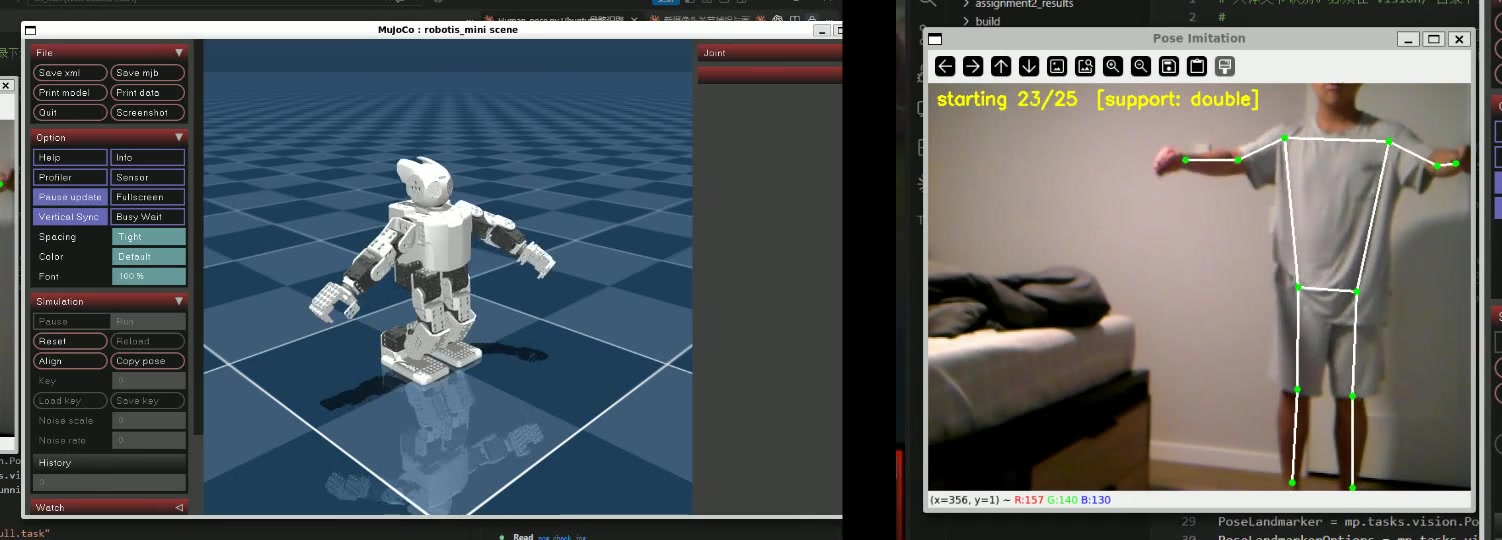
\includegraphics[width=0.49\textwidth]{figures/sim_tpose.jpg}\hfill
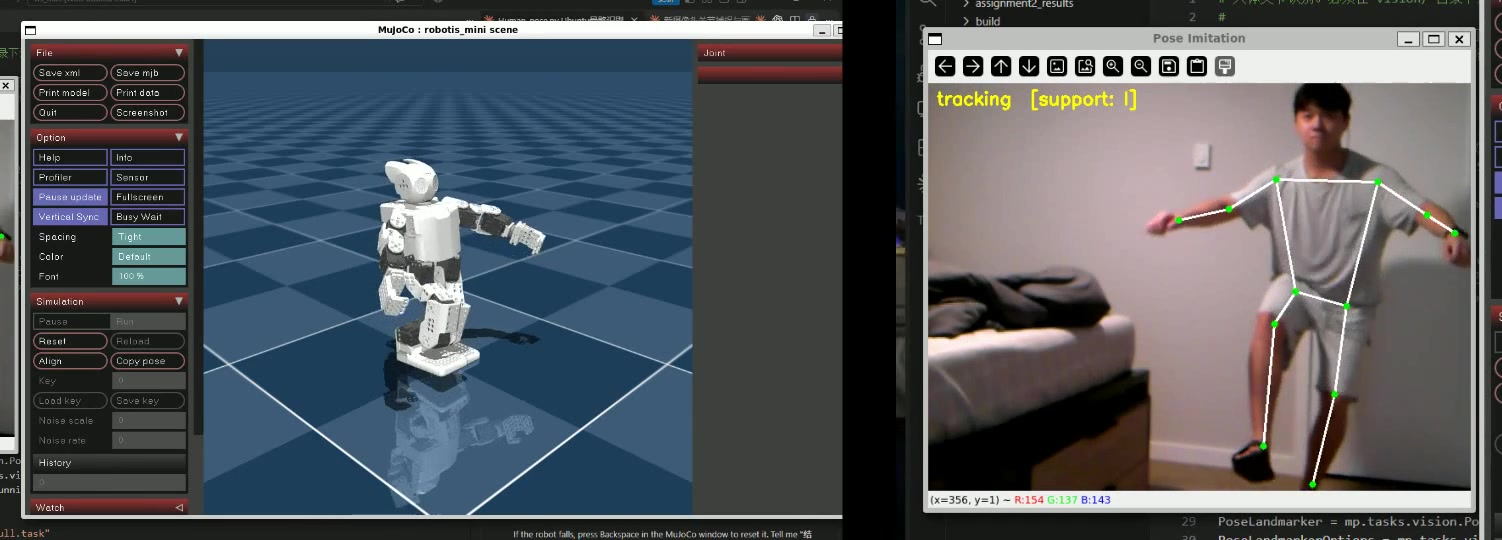
\includegraphics[width=0.49\textwidth]{figures/sim_knee_left.jpg}\\[4pt]
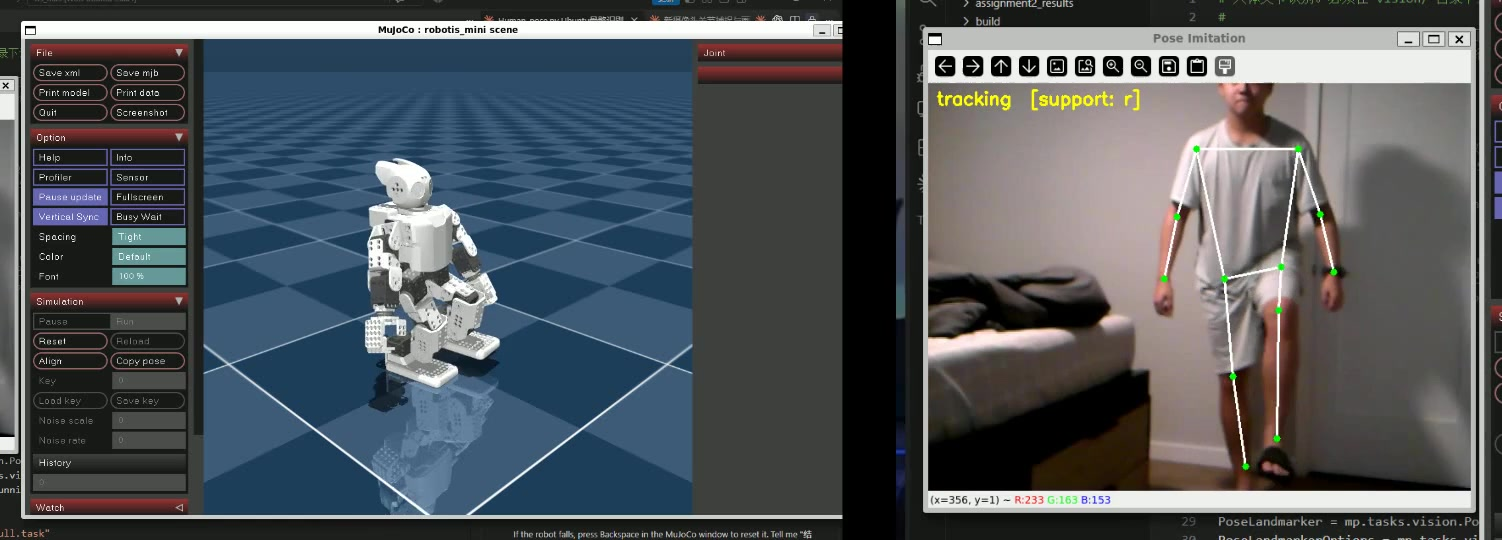
\includegraphics[width=0.49\textwidth]{figures/sim_knee_right.jpg}\hfill
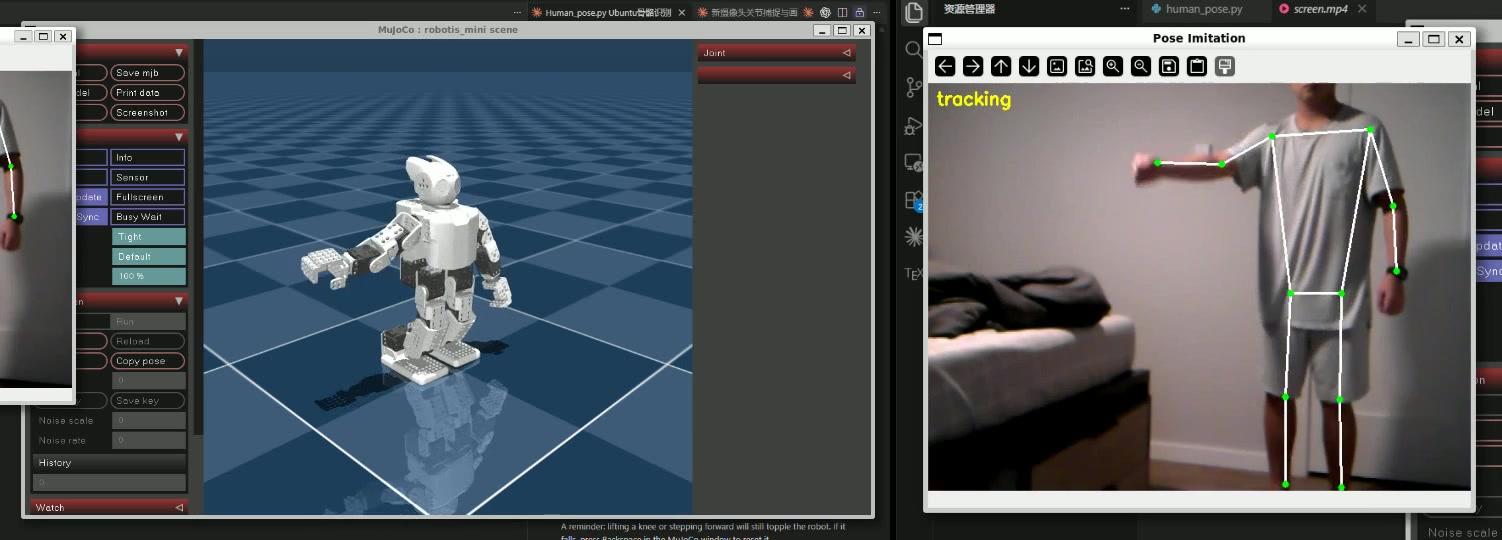
\includegraphics[width=0.49\textwidth]{figures/sim_arm_nofilter.jpg}
\caption{仿真运行截图。左上：启动过渡（\code{starting}），T 字姿势；右上：左脚支撑（\code{support: l}），机器人先移重心再抬腿；左下：右脚支撑（\code{support: r}）；右下：加过滤之前的运行，单臂侧平举。}
\label{fig:sim}
\end{figure}

%=====================================================================
\section{真机}

\subsection{硬件组成}
真机是装有 KIMLAB MINI 升级套件的 Robotis MINI：
\begin{itemize}
  \item 16 个 Dynamixel XL-320 舵机（Protocol 2.0，1 Mbps，位置 0–1023，每单位 0.293°，力矩上限 0.39 Nm），ID 1–16，奇数为右侧、偶数为左侧；
  \item U2D2 USB 串口转接器（FTDI 芯片），连接到舵机总线；
  \item Orange Pi Lite 2 单板电脑、BNO055 IMU、头部 USB 摄像头（本阶段未使用）；
  \item 电源分配板，两节 3.7 V 锂电池串联（满电约 8.4 V），或 7.5 V 电源适配器。
\end{itemize}

\subsection{连接方式}
套件中 U2D2 的 USB 默认接在 Orange Pi 上。为了先在笔记本上调试，把 U2D2 的 micro USB 改接到笔记本（注意要用能传数据的线，只能充电的线电脑认不到），然后：
\begin{Verbatim}
usbipd bind --busid <BUSID> --force   # 管理员 PowerShell，只需做一次
usbipd attach --wsl --busid <BUSID>   # 每次插拔后做一次；BUSID 用 usbipd list 查
# 把 U2D2 的延迟参数从 16 ms 调到 1 ms：
echo 1 | sudo tee /sys/bus/usb-serial/devices/ttyUSB0/latency_timer
\end{Verbatim}
挂载后 WSL 里出现 \code{/dev/ttyUSB0}。用户需要加入 \code{dialout} 组才有串口权限。U2D2 本身由 USB 供电，但舵机要接上电池或适配器才能应答。

\subsection{校准}
\begin{enumerate}
  \item \textbf{扫描}（\code{tools/dxl_scan.py}，只读）：1 Mbps 下 16 个舵机全部在线，均为 XL-320，电压 7.4–8.0 V，温度 26 °C。
  \item \textbf{方向}（\code{tools/dxl_joint_test.py}）：机器人悬空，每次只给一个舵机开力矩，转动 10°–15° 再转回，对照仿真模型算出的预期动作目测方向。结果：\textbf{ID 1、2（两个肩关节）与仿真相反，其余 14 个一致}。
  \item \textbf{零点}（\code{tools/dxl_pose_test.py zero}）：16 个关节同时转到 0°，实际位置与目标的偏差都在 2.1° 以内，外观与仿真的 0° 姿势（手臂水平侧举、腿伸直、脚底平）一致，零点不需要调整。
\end{enumerate}
校准结果保存在 \code{config/real_robot_calibration.yaml}：舵机位置 $=$ 512 $+$ 方向 $\times$ 角度(rad) $\times$ 195.38。

\subsection{真机桥接节点}
\code{real_robot_bridge.py} 订阅与仿真器相同的命令话题，所以模仿节点无需修改：
\begin{itemize}
  \item 每秒 50 次用 Sync Write 同时发送 16 个目标位置，每秒 10 次读回实际角度并发布 \path{/robotis_mini/joint_states}；
  \item \textbf{启动}：先把目标设为当前位置再开力矩（不会突然跳动），然后用 3 秒慢慢移到默认站姿；
  \item \textbf{限位与限速}：每个关节按仿真范围限位，最快 2 rad/s；
  \item \textbf{电压与温度保护}：每秒检查一次。电压取 16 个舵机的中位数，连续 3 秒低于 6.3 V 才停机（舵机用力时总线电压会比静置时低 0.5–1 V，单次读数或瞬间下降不应触发停机）；任一舵机超过 65 °C 也停机；
  \item \textbf{退出}：任何原因退出都会关闭全部力矩。机器人站着时，关闭力矩后会变软，所以退出前要扶住。
\end{itemize}

\subsection{运行方法}
\begin{Verbatim}
cd ~/ws_mini && source devel/setup.bash
roslaunch final_project real_imitation.launch camera_source:=0 imitate_legs:=true
\end{Verbatim}
真机启动文件默认只模仿手臂（\code{imitate_legs:=false}），需要全身模仿时显式打开。第一次运行时机器人应保持悬空；出现异常时最快的急停方法是拔掉电源。\code{tools/replay_commands.py} 可以不开摄像头，按原节奏重放录下的命令（可只重放手臂），用来先检查动作。

\subsection{运行结果}
\begin{table}[H]
\centering\small
\begin{tabularx}{\textwidth}{lY}
\toprule
运行 & 结果 \\
\midrule
\code{real_20261031_185703} & 完整运行 77 s，手动结束。识别 18.5 fps；第 4.0 s 开始等待全身入镜，30.3 s 开始过渡，32.0 s 进入跟踪；正常跟踪 647 帧（约 45 s），其中 19 帧单脚支撑。舵机工作时总线电压 6.8–7.0 V，温度最高 32 °C，通信没有中断。 \\
\code{real_20261031_185928} & 运行约 56 s 后，总线电压连续 3 s 为 6.2 V，桥接节点按设计自动停机并关闭力矩。之后测得静置电压中位数 7.3 V（每节约 3.65 V，剩余约 30–40\%）。 \\
\bottomrule
\end{tabularx}
\caption{真机运行记录}
\end{table}
\noindent 两次真机运行都没有录屏，机器人实际动作的外观（方向、幅度是否自然）本文没有记录，需要在后续测试中补充视频。

%=====================================================================
\section{已知限制与后续工作}
\label{sec:limits}
\begin{itemize}
  \item \textbf{快速起身}：从深蹲快速站起（不到 1 秒）时，膝关节力矩跟不上，机器人会向后倒。可以限制着地腿的伸膝速度，并把下蹲上限从 30° 再收紧到约 25°。
  \item \textbf{静态过滤}：重心过滤只做静态检查，不处理动作过程中的惯性和晃动。下一步可以用 IMU（仿真中已有，真机套件中有 BNO055）根据躯干实际倾斜实时修正踝关节和髋关节。
  \item \textbf{上身前倾}：机器人上身始终直立，不模仿人的弯腰；弯腰时由下蹲限制和重心过滤保证安全。
  \item \textbf{手臂结构}：MINI 的手臂做不出“上臂下垂、前臂向前”的动作。
  \item \textbf{真机供电}：电池剩余 30–40\% 时，舵机用力会让总线电压降到 6.2 V 左右，接近 XL-320 的最低工作电压。长时间调试建议使用 7.5 V 电源适配器（2.5$\times$5.5 mm，至少 2 A）。
  \item \textbf{无线化}：目前 U2D2 通过 USB 接在笔记本上。之后可以把桥接节点放到机身上的 Orange Pi 运行，笔记本通过 Wi-Fi 用 ROS 发送命令。
  \item \textbf{识别速度}：两次保留的仿真录制中识别只有每秒 13.4 帧和 11.0 帧，真机运行（未录屏）为 18.5 帧。推测是录屏和仿真占用了 CPU，但没有单独验证。
\end{itemize}

%=====================================================================
\section{工具}
\label{sec:tools}
\begin{table}[H]
\centering\small
\begin{tabularx}{\textwidth}{>{\ttfamily}p{4.6cm}Y}
\toprule
\normalfont 工具（\code{tools/}） & 作用 \\
\midrule
record\_windows.py & Windows 端录制 MuJoCo 和摄像头两个窗口（置顶并排），输出 mp4，需再用 ffmpeg 转成 H.264 \\
extract\_bag.py & 把录制目录里的 rosbag 提取成 npz \\
analyze\_run.py & 分析一次仿真录制：延迟、平滑、关节跟随、站立情况 \\
export\_mass\_model.py & 从 MuJoCo 模型导出重心过滤用的质量参数 \\
test\_balance\_filter.py & 重心过滤的仿真回归测试（配合 synthetic\_human.py） \\
dxl\_scan.py & 扫描舵机：ID、型号、位置、电压、温度（只读） \\
dxl\_joint\_test.py & 单关节方向测试 \\
dxl\_pose\_test.py & 全身转到指定姿势（0° 或默认站姿） \\
joint\_test\_plan.py & 用仿真算出每个关节测试时的预期动作 \\
replay\_commands.py & 按原节奏重放录下的关节命令 \\
\bottomrule
\end{tabularx}
\caption{辅助工具}
\end{table}

%=====================================================================
\newpage
\section{录制数据}
保留的录制数据打包在 \code{recordings.zip} 中（运行失败、没有有效数据的 3 次真机记录已删除）：
\begin{table}[H]
\centering\small
\begin{tabularx}{\textwidth}{>{\ttfamily}p{4.4cm}Y}
\toprule
\normalfont 目录 & 内容 \\
\midrule
20261031\_170832 & 仿真，加重心过滤之前。延迟分析的数据来源；含第 56 s 弯腰摔倒。录屏 55 s（\code{screen.mp4}） \\
20261031\_174418 & 仿真，加重心过滤之后。抬膝、下蹲；录屏 44 s（原始第 9–53 s） \\
real\_20261031\_185703 & 真机，完整运行 77 s \\
real\_20261031\_185928 & 真机，运行 56 s 后因电池电压低自动停机 \\
\bottomrule
\end{tabularx}
\caption{保留的录制数据}
\end{table}
\noindent 每个目录中：\code{frames.npz} 是每帧数据（关键点、处理耗时、丢弃的旧帧数、过滤前后的关节命令、支撑状态）；仿真目录另有 \code{robot.bag}（关节角、躯干姿态、命令）、\code{robot_extracted.npz} 和录屏 \code{screen.mp4}（H.264）；\code{launch.log} 等是运行日志。录屏只剪辑了视频，数据文件保留完整运行。

%=====================================================================
\section{常见问题}
\begin{table}[H]
\centering\small
\begin{tabularx}{\textwidth}{p{4.6cm}Y}
\toprule
现象 & 原因与解决 \\
\midrule
没有 \code{/dev/video0} & 摄像头没挂进 WSL：\code{usbipd attach --wsl --busid 1-3} \\
读帧超时（select timeout） & 确认程序设置了 MJPG 格式 \\
外接摄像头画面绿屏 & 该摄像头不能经 usbip 使用，改用 Windows 推流 \\
推流显示已连接，但窗口不出现 & wslrelay 没有转发：推流时传 WSL 的 IP，不要用 127.0.0.1 \\
延迟越来越大 & 接收端必须只取最新一帧（当前代码已处理） \\
电脑认不到 U2D2 & 线是只能充电的线，换数据线；或 U2D2 仍接在 Orange Pi 上 \\
U2D2 在，但点名不到舵机 & 机器人没有通电（舵机需要电池或适配器供电） \\
偶发 “no status packet” & USB 透传偶发丢包，工具和桥接节点都会自动重试 \\
桥接节点因电压停机 & 电池电量低或负载下电压下降过多，充电或改用 7.5 V 适配器 \\
\bottomrule
\end{tabularx}
\caption{常见问题排查}
\end{table}

\end{document}
